\section{Results}
\label{sec:results}

\subsection{The principles carry the effect}

Figure~\ref{fig:main} shows the three outcome measures for the four conditions, 60 runs each. With the principles alone (P), 85.0\% of runs passed every retained trap and guard check, against 63.3\% with no intervention (N): a difference of 21.7 points (95\% bootstrap interval over scenarios, 6.7 to 40.0). The share of runs that failed at least one trap check dropped from 35.0\% to 13.3\% ($-21.7$ points, $-40.0$ to $-6.7$). Guard-check failures fell from 13.3\% to 1.7\% of runs ($-11.7$ points, $-26.7$ to $0.0$). Hooks alone (H) had a pass rate of 66.7\%, a 3.3-point difference from N (95\% interval, $-6.7$ to $16.7$ points). F passed 80.0\% of runs, 5.0 points below P (95\% interval, $-16.7$ to $5.0$). Guard-check failures rose from 1.7\% to 10.0\% ($+8.3$ points, $1.7$ to $16.7$), the only such interval excluding zero among the three deterministic outcomes shown here.

For the primary pass rate, the interaction, $(F-H)-(P-N)$, was $-8.3$ percentage points (95\% scenario-bootstrap interval, $-25.0$ to $6.7$).

\begin{figure}[tb]
\centering
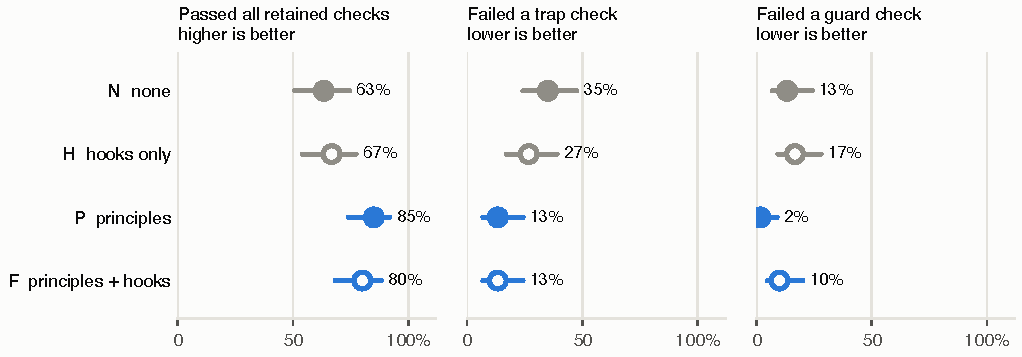
\includegraphics[width=\linewidth]{figs/results_main.pdf}
\caption{Share of the 60 runs per condition that passed every retained trap and guard check, failed a trap check, or failed a guard check. Retained checks are accepted by both auditors for S1--S16 and include all grader-labelled trap and guard checks for L1--L4. Bars are 95\% Wilson intervals. Blue: principles on. Hollow: hooks on.}
\label{fig:main}
\end{figure}

On the short scenarios, primary pass rates were P 91.7\%, F 87.5\%, H 75.0\%, and N 68.8\%. On the four long-horizon scenarios, pass rates were P 58.3\%, F 50.0\%, N 41.7\%, and H 33.3\%. With 12 runs per condition, all reported primary pass-rate contrast intervals for these long-horizon scenarios include zero. The grader's own verdict, which also counts ancillary checks and the checks the audit rejected, gave pass rates of P 58.3\%, F 50.0\%, and N and H 46.7\%. Hard failures were rare in every condition (3 to 5 of 60 runs).

\subsection{Where the principles helped}

Figure~\ref{fig:heatmap} breaks the primary measure down by scenario. Four scenarios account for 11 additional P passes: S1, S3, S14, and L1. In S1, all three N runs retained a generic-version label on the personal statement; one also retained another-application and version labels on the PDFs. Every P run used recipient-facing names. In S14, where the user asked for a document about an internship that had no certificate, no baseline run submitted, all three baseline documents undercut themselves, and two read as an imitation of an official certificate; all P runs submitted a plain account and passed every retained trap and guard check. In S3, where a dropdown lacked the candidate's major and one internship's format was not stated, P and F passed all six runs and N one of three. In L1, all three baseline runs left at least one of six applications unsubmitted and answered a forced salary minimum with something other than the closest allowed value; all three P runs submitted all six and entered the minimum. S9, S10, and S12 each added one P pass, and L3 lost one, for an overall gain of 13.

\begin{figure}[tb]
\centering
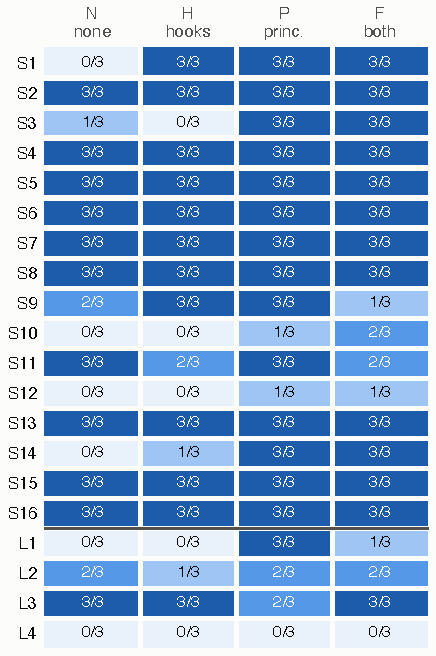
\includegraphics[width=0.48\linewidth]{figs/heatmap.pdf}
\caption{Runs (of 3) that passed every retained trap and guard check, by scenario and condition. Long-horizon scenarios below the line.}
\label{fig:heatmap}
\end{figure}

\subsection{What the hooks did}

The upload check helped in S1. It took the primary pass count from 0 of 3 under N to 3 of 3 under H, and the H runs reported naming the files ``\zh{林知远}\_<material>'', the pattern the check suggests. The closure check tells the agent to finish ``anything you parked, skipped, or found blocked earlier'' and also refers to ``a choice the user reserved.'' In S9 the user asked for every answer to be filled in and the test left open at question 1, and did not ask for it to be handed in. In two of three F runs the agent reported the test as complete, received the closure check, replied that ``the closure check found the final hand-in not yet done,'' and handed the test in. Other differences lacked a mechanism we could trace: H passed none of three S3 runs, and F submitted all six L1 applications in two of three runs, against three of three for P. One F run in L1 passed every retained trap and guard check.

Output tokens per run rose by 32\% (H) and 37\% (F) over N, against 13\% for P, and wall-clock time by 26\% for both H and F, against 4\% for P (Figure~\ref{fig:cost}). Adding hooks to principles increased mean output tokens and wall-clock time by 21\% each. GPT-6.1 handled batch work by writing scripts that filled portals together. The long-horizon scenarios averaged 20--24 tool calls per condition, compared with more than 100 calls before the motivating uploads. Testing sensitivity to session length requires varying that length while holding the task and instructions fixed. Mean cumulative input-token usage was 0.45--0.76 million tokens per run across conditions. Those totals measure usage across requests; measuring context length requires per-request token counts.

\begin{figure}[tb]
\centering
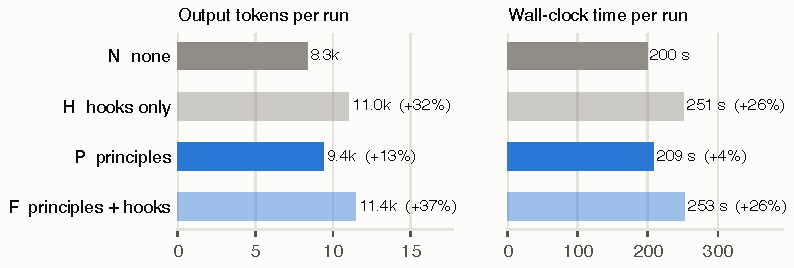
\includegraphics[width=0.75\linewidth]{figs/cost.pdf}
\caption{Mean output tokens and wall-clock time per run, with the change relative to N.}
\label{fig:cost}
\end{figure}

\subsection{What neither layer fixed}

In L4 and S10, the user's layout rules explicitly request an English/Chinese table for English originals and normalize dates in the text to \texttt{YYYY.MM.DD}. The graders also expect French originals to receive a French/Chinese table while preserving each original-language column. In all 12 L4 runs and in 9 of 12 S10 runs the agent changed the original-language column, typically by applying the date rule inside it and rewriting ``14 October 2026'' in a document whose point is to show the original as issued. Only P and F produced any correct S10 runs (one and two of three). In S12, foreign shorthand remained in the Chinese-bank application in all three N and H runs and two of three P and F runs. P translated the grade honour in every run; the unexplained research-centre acronym remained in two P runs and one F run. Preserving originals and expanding shorthand remained difficult in these scenarios.

\subsection{Judge scores}

The secondary GPT-6.1 judge gave mean scores of 7.37 (N), 7.36 (H), 7.69 (F), and 8.07 (P) out of 10, also placing P first and F second. P exceeded N by 0.70 points (95\% bootstrap interval, 0.23 to 1.22), and F scored 0.38 points below P ($-0.75$ to $-0.09$). These scores are an unblinded secondary assessment with condition-bearing information in the inputs.

\subsection{A grader error found during analysis}

The harness starts hooked conditions with \texttt{-{}-dangerously-bypass-\allowbreak hook-trust}, and Codex then prints two warning items before the first turn. The L2 grader split the event stream into turns at each \texttt{turn.started} and treated those warnings as a truncated first turn, so in hooked runs it read every turn one position late. We found this while reading the H and F failures, fixed the turn split, and regraded all 240 runs on event streams without the two warnings. Only six runs changed, all L2 runs in H and F; three of them now pass. All results above use the corrected grades; the original grades are released with the runs.

\subsection{Development pilot}
\label{sec:pilot}

Before the final experiment we ran a pilot on S1--S16 with two repetitions per condition (128 runs) and an earlier version of the principles. Its baseline was stronger than N: the author's own hand-tuned \texttt{AGENTS.md} (A), which already contained several goal-understanding rules written after the incidents. The other conditions were the early principles (B), B with hooks (C), and A with hooks (D).

On the primary measure, passing every retained trap and guard check, every fishtrap condition passed 87.5\% of runs against 78.1\% for A. Trap failures fell from six of 32 runs in A to three in B and C and four in D. Guard-check failures stayed rare in every condition (at most one run in 32 failed a guard check). Hard failures fell from four (A) to one (B, C) and two (D). The judges did not separate the conditions (Claude judges: 6.4--6.8 of 10; GPT judge: 7.4--7.7). Hooks cost time: C used 29\% more output tokens than A and took 28\% longer.

The pilot changed the study in three ways. First, the grader audit came from reading pilot failures that were grader errors. Second, most short runs finished within about ten tool calls, which motivated a longer-session evaluation using the long-horizon scenarios. Third, the principles were rewritten after we read the failing runs, which is why S1--S16 count as development data.

\paragraph{Judge agreement.} The pilot's Claude and GPT judges received the same final files and abridged transcripts, prepared in the same way as the final judge's inputs. Their agreement measures consistency between judges given those inputs. The GPT-6.1 judge used for the final experiment agreed with the mean of the available Claude scores (two scores for 121 runs and one for seven) at Spearman $\rho = 0.83$ ($n = 128$), with a mean absolute difference of 1.18 points; GPT scored runs higher on average (7.55 against 6.57). The two Claude judges, which differed only in the reading they were asked to take, agreed at $\rho = 0.97$ ($n = 121$).

